\documentclass{ltjsarticle}

\usepackage{amsmath}
\usepackage{amssymb}
\usepackage{amsthm}
\usepackage{ mathrsfs }
\usepackage{enumerate}
\usepackage{bbm}
\usepackage{lipsum}
\usepackage{fancyhdr}
\usepackage{tikz-cd} 
\usetikzlibrary{graphs}
\usepackage{luatexja-ruby} 
\usepackage{graphicx} 
\graphicspath{ {./../../images/} }

\newtheorem{theorem}{定理}
\newtheorem{proposition}{Proposition}[section] 
\newtheorem{definition}{定義}
\newtheorem{problem}{問題}
\newtheorem{postulate}{公準}[section] 
\newtheorem{lemma}{Lemma}[section] 
\newtheorem{notation}{Notation}[section] 
\newtheorem{remark}{注釈} 
\newtheorem{corollary}{系}[section] 
\newtheorem{terminology}{Terminology}[section] 
\newtheorem{example}{例}
\newtheorem{step}{手順} 
\newtheorem{solution}{解答}[section] 
\newtheorem{fact}{事実}[section] 
\newtheorem{exercise}{問題}


\DeclareMathOperator{\diam}{diam}
\DeclareMathOperator{\Gal}{Gal}
\DeclareMathOperator{\rank}{rank}
\DeclareMathOperator{\Hom}{Hom}
\DeclareMathOperator{\Dom}{Dom}
\DeclareMathOperator{\Ann}{Ann}
\DeclareMathOperator{\grad}{grad}
\DeclareMathOperator{\Span}{Span}
\DeclareMathOperator{\interior}{int}
\DeclareMathOperator{\ind}{ind}
\DeclareMathOperator{\supp}{supp}
\DeclareMathOperator{\ob}{ob}
\DeclareMathOperator{\Spec}{Spec}
\DeclareMathOperator{\MaxSpec}{MaxSpec}
\DeclareMathOperator{\PreSh}{PreSh}
\DeclareMathOperator{\Sh}{Sh}
\DeclareMathOperator{\Fun}{Fun}
\DeclareMathOperator{\Ext}{Ext}
\DeclareMathOperator{\Aut}{Aut}
\DeclareMathOperator{\Ker}{Ker}
\DeclareMathOperator{\Image}{Im}
\DeclareMathOperator{\Coker}{Coker}
\DeclareMathOperator{\id}{id}
\DeclareMathOperator{\Mod}{Mod}
\DeclareMathOperator{\QCoh}{QCoh}
\DeclareMathOperator{\Coh}{Coh}
%\newcommand*{\name}[\num_arguments][default values]{{\color{#1}\Large #2}}
\newcommand*{\Z}{\mathbb{Z}}
\newcommand*{\Q}{\mathbb{Q}}
\newcommand*{\R}{\mathbb{R}}
\newcommand*{\multivar}[2]{{#1_1,\cdots,#1_{#2}}}
\newcommand*{\localization}[2]{#1_{\mathfrak{#2}}}
\newcommand*{\ringedspacemorph}[1]{(#1,#1^{\#})}
\newcommand*{\sheaf}[2]{(#1,{\mathcal{#2}}_{#1})}
\newcommand{\fib}[1]{%
  \mathbin{\mathop{\times}\limits_{#1}}%
}
\newcommand{\tens}[1]{%
  \mathbin{\mathop{\otimes}\displaylimits_{#1}}%
}
\title{グラフ理論プリント}
\author{ボン補習校高校数学}
\date{}

\begin{document}

\maketitle

\begin{definition}
グラフの部分グラフ要するに、元のグラフから必要な頂点を辺を選んで作ったグラフのことである。
\begin{center}
\begin{figure}[h]
	\centering
    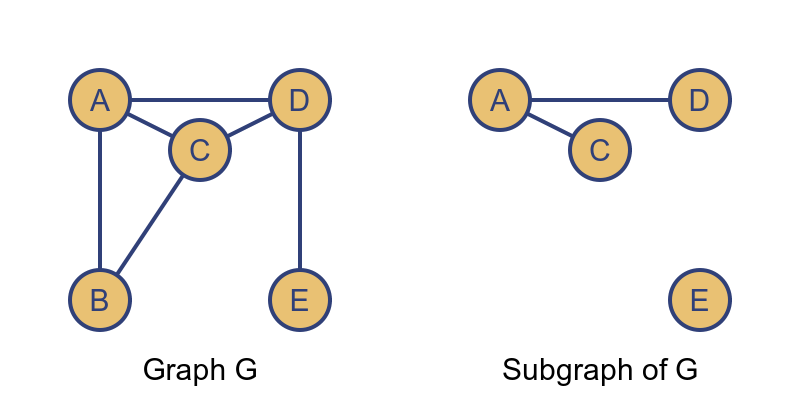
\includegraphics[scale=0.3]{subgraph}
    \label{fig:subgraph}
    \caption{部分グラフの例}
\end{figure}
\end{center}
\end{definition}

\begin{definition}
どんな二つの頂点においても二つをつなぐ道が部分グラフとしてあるときに、このグラフを連結グラフという。また繋がっている頂点を全てまとめた誘導部分グラフを連結成分という。
\begin{center}
\begin{figure}[h]
	\centering
    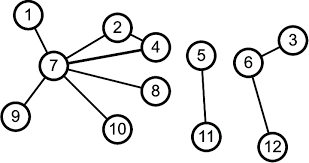
\includegraphics[scale=0.5]{components}
    \caption{このグラフは三つの連結成分よりなる}
    \label{fig:connected_components}
\end{figure}
\end{center}
\end{definition}


\begin{definition}
連結グラフがサイクルを部分グラフとしてもたないとき、これを木という。
\begin{center}
\begin{figure}[h]
	\centering
    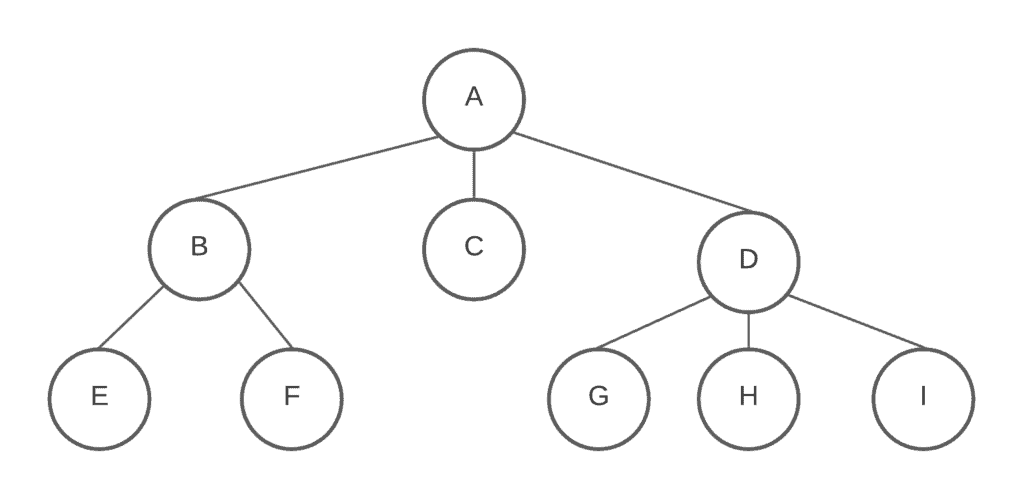
\includegraphics[scale=0.2]{tree}
    \caption{木の例}
    \label{fig:tree}
\end{figure}
\end{center}
\end{definition}
\begin{remark}
木の便利な性質の一つに、新しい辺を足すとサイクルができることです。例えば$E,F$に辺を足すと$B,E,F$が閉路グラフ$C_3$となります。これはどの二つの頂点の間にも道が存在するので、辺を足すことは道の両端を足す、つまりサイクルを作り出します。
\end{remark}


\begin{example}
最も単純な例として、全て道は木である。
\end{example}

\begin{definition}
あるグラフの\ltjruby{全域木}{ぜんいきぎ}とは木である部分グラフで全ての頂点を含むものである。
\begin{center}
\begin{figure}[h]
	\centering
    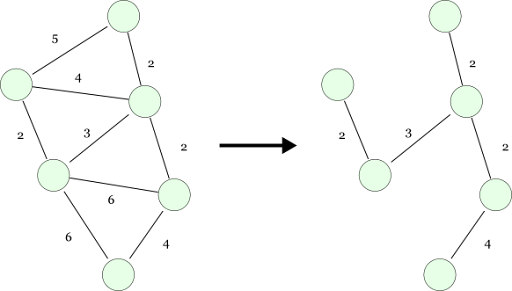
\includegraphics[scale=0.5]{spanning_tree}
    \caption{全域木の例}
    \label{fig:spanning_tree}
\end{figure}
\end{center}
\end{definition}

微分積分で習った数学的帰納法のおさらいをしましょう。数学的帰納法とはある命題が
\begin{enumerate}[i).]
\item $n=1$の時成り立つ、
\item $n-1$の時成り立つなら$n$の時も成り立つ、
\end{enumerate}
を満たす時、その命題は全ての自然数に対して成り立つというものでした。重要なのは何を$n$とするかです。これを使って次のことを証明します。

\begin{theorem}
連結グラフはかならず部分グラフで全域木となるものがある。
\end{theorem}

\begin{proof}
連結グラフ$G=(V,E)$を考えます。ここで我々が$n$とするのは頂点の個数です。
\par $n=1$、すなわち頂点の個数が$1$のとき、このグラフは単純グラフなので
\begin{center}
\begin{figure}[h]
	\centering
    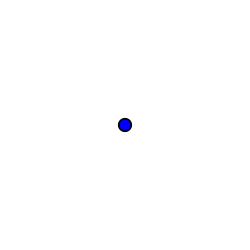
\includegraphics[scale=0.3]{single_vertex}
    \caption{頂点が一つしかないグラフ}
    \label{fig:single_vertex}
\end{figure}
\end{center}
このように辺が存在できません。もしあるなら自分自身を繋げるループになってしまいます。よってそのグラフ自身が木となります。
\par $n-1$のとき成り立つとします。$V=\{1,2,\cdots,n-1,n\}$の$n$個の頂点があるグラフを考えます。$n$番目の頂点を除いた誘導部分グラフを考えます。これは$n-1$この頂点を持つグラフなので全域木が存在します。この部分グラフを$T$とします。この$T$はもちろん$G$の部分グラフでもあります。$G$は連結なので$n$は必ず$T$のどこかの頂点と繋がっています。そのような頂点を一つ選んで$n$と繋がっている辺を追加したグラフ$T'$を考えます。すると$T'$は木となります。よって数学的帰納法により命題が成り立ちます。
\end{proof}

\begin{definition}
木において、次数が$1$の頂点を\ltjruby{葉}{は}という。
\end{definition}
\begin{example}
図３の木において$E,F,G,I,H$が葉。
\end{example}

\begin{exercise}
木は必ず葉を持つことを示せ。
\end{exercise}

ヒント、道の葉を考えてみよう。グラフの中の二つの頂点の間には必ず道が見つかる。頂点が葉ではない時別の頂点を見つけて道を長くすることはできるだろうか。逆に葉のときは道はどうなるだろうか。頂点の個数が有限なことにも注意しよう。

\begin{exercise}
全ての頂点が偶数の連結グラフの中には必ず閉路グラフがあることを示せ。
\end{exercise}

ヒント：葉の次数は幾つだっただろうか。葉と別の頂点を繋げる辺は元のグラフに存在するだろうか。


\end{document}